
%%% Local Variables: 
%%% mode: latex
%%% TeX-master: t
%%% End: 


\documentclass{sig-alternate}

% Housekeeping
% Proudly writing in Emacs with TeXLive 2012 under Debian 7.3.
\usepackage{amsmath}
\usepackage{amssymb}

\usepackage{cite}
\usepackage{algorithmic}
\usepackage{array}
\usepackage{graphicx}
\graphicspath{{./}{./Figure/}}

\usepackage{url}





% This should be put last.
\usepackage{hyperref}





\begin{document}
\title{Improving Building Energy Efficiency by Kinect-based Occupancy
  Tracking and Mobility Detecting System}

\numberofauthors{1}
\author{
\alignauthor
Haleimah Al Zeyoudi\quad Yanan Xiao\quad Chi-Kin Chau\\
\affaddr{Masdar Institute of Science and Technology}
\affaddr{P.O. Box 54224}
\affaddr{Abu Dhabi, UAE}
\email{\{hzeyoudi,yxiao,ckchau\}@masdar.ac.ae}
}

% \numberofauthors{1}
% \author{
% \alignauthor
% Some author
% }


\maketitle{}



\begin{abstract}
  Nowadays, most building air conditioning systems still operate on a
  fixed schedule rather than real-time occupancy states. In our study, we
  make an occupancy tracking software based on Kinect to reflect the
  number of people in a open lab. We then build a Markov Chain (MC)
  model after dividing the open area into 4 zones and calculating its
  occupancy respectively. When applying the real-time schedule
  generated from MC model to a building model created with eQuest, we
  obtain a 22.1\% energy reduction in space cooling. 
\end{abstract}

% I comment out this part. It seems that it's useless.

% \category{C.3}{Special-purpose and application-based
%   systems}{Real-time and embedded systems}

% \terms{Algorithms, Design, Management}

% \keywords{Wireless sensor networks, Markov chain, Simulation}





% What the heck am I reading.


\section{Introduction}
\label{sec:introduction}
At the core of energy consumption in
modern buildings is Heating Ventilation and Air Conditioning (HVAC)
systems which are designed to operate at full capacity most of the
time because it's often assumed a maximum occupancy, according
to~\cite{ref:Wang2011}. Although current HVAC systems are equipped with sensors, their management and control
systems ignore the dynamic nature occupancy patterns in buildings. In
addition, they are unable to proactively adjust to occupants' comfort
levels. Understanding human mobility and occupancy patterns are key
factors in successfully managing HVAC systems in buildings. The main
contribution of our paper is to propose an energy-saving model based
on occupancy patterns of human mobility in buildings. The most
important features of the system are as follows: a) A real-time
detection and tracking of human mobility in buildings based on
Kinect; b) An occupancy prediction mechanism based on MC. 
% This part should be concised.
\par






\section{Implementation}
\label{sec:implementation}

\subsection{Kinect-based Occupancy Counting Software}
Our occupancy counting software is written using Microsoft Visual
C\# 2010, project WPF application in C\# and XML\@. Both types of
Kinect are used and tested to insure that it works fine, i.e. Xbox
Kinect and Kinect for Windows. The software, should be run on windows
7 or above, after a successful installation of Kinect drivers.    
\par
% In the next paragraph I would sum up the functions of this software
% and some extras behind it.

Once the software is started, it will do self-diagnosis to check
if a Kinect is connected to the computer properly. Then both the red,
green and blue (RGB) and depth images are captured with the help of
color sensor as well as infrared (IR) sensor, which comes with
Kinect. The depth image as shown in Figure~\ref{fig:system-arch}. For
each depth image captured, a corresponding blue box with unique ID is
drawn to detect the movement of multiple people at the same time. We
implement both human posture tracking and skeletal tracking for the
sake of a higher detection accuracy. Reference code of the latter can
be found in MSDN library.

\subsection{Testbed Setup}
\label{sec:testbed-setup}

The environment we have is an open laboratory with no doors separating
each professor's office. Therefore we divide this lab into 4 zones and
deploy 8 Kinect sensors along with a cheap laptop running Windows at
key areas of each zone, i.e.\ the conceptual entrance and exit. The in
and out image is captured by Kinect and processed in Windows. All the
in and out data is stored in laptops and synchronized via Dropbox. A
selection of deployments is shown in Figure.


\begin{figure}[!tb]
  \centering
  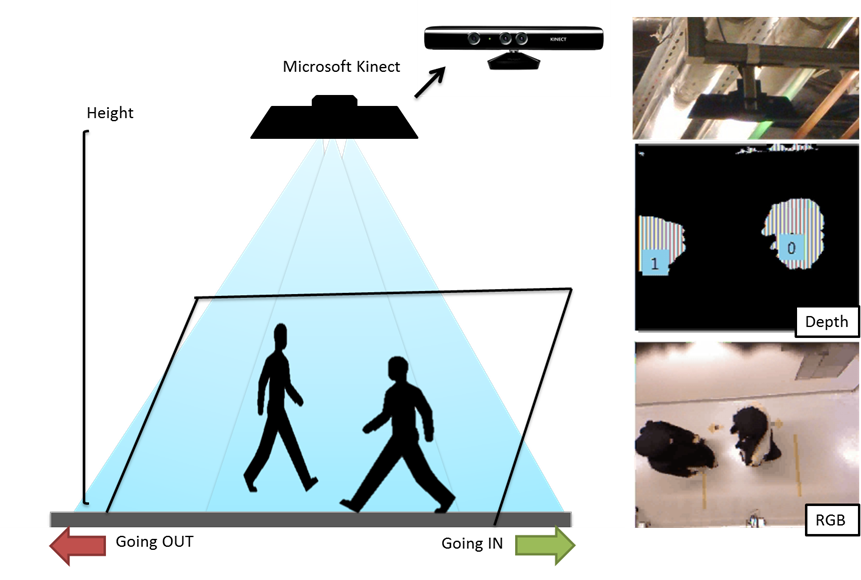
\includegraphics[scale=0.5]{minisys}
  \caption{Architecture of human mobility tracking system}
  \label{fig:system-arch}
\end{figure}

\begin{figure}[!tb]
  \centering
  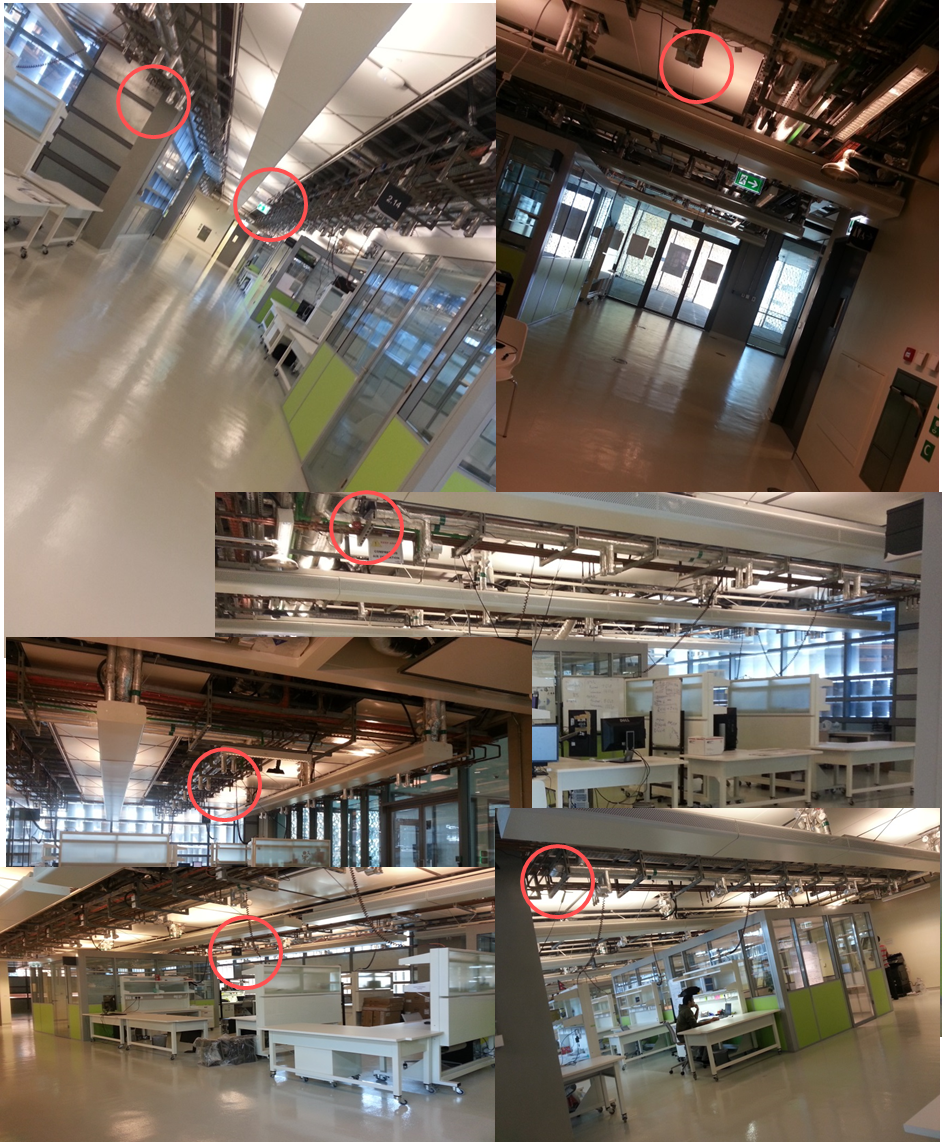
\includegraphics[scale=0.3]{realworld}
  \caption{Kinect deployments in an open lab}
  \label{fig:kinect-deployment}
\end{figure}



\subsection{Markov Chain Prediction Model}
\label{sec:mark-chain-pred}

% Life is never easy. Especially when you are a graduate student.
We decide to use MC to build our prediction model after comparing
results
in~\cite{ref:Erickson:2009,ref:Erickson:2010}. We start by parsing in
and out log files into occupancy files, and then inspect the
distribution of occupancy data, i.e.\ number of people at a specific
time slot in each zone. We adopt a time slot of 30min in the end and
scale the occupancy data down into 4 states: E for empty, F for few, M
for medium and C for crowded. For each time slot, one and only one
occupancy state is assigned with respect to the number of people in
that zone. For example, when the number lies in between 8 and 14, then
the state is marked M.
\par
% In this part we will describe how the transition matrix is built and
% how it ``seemingly'' works.
Judging from the high accuracy of our Kinect detection system, which
we conclude by manually counting the captured videos and comparing
with software-generated data, we use the occupancy data alone to train
Markov model. Briefly speaking it is a 256-by-256 matrix due to the
fact that we use a zone-based method to deal with this open lab, and
each zone may be at one of four states when doing the permutation.
\par
The matrix we get is extremely sparse because most of the states and
the next state to which it will jump do not exist in reality. The
simplified states and their transitional relations are shown in
Figure~\ref{fig:transitional-matrix}. This transitional relation is
then used to build a dynamic control system with which the ventilation
and air conditioning systems are adjusted.

\begin{figure}[!tb]
  \centering
  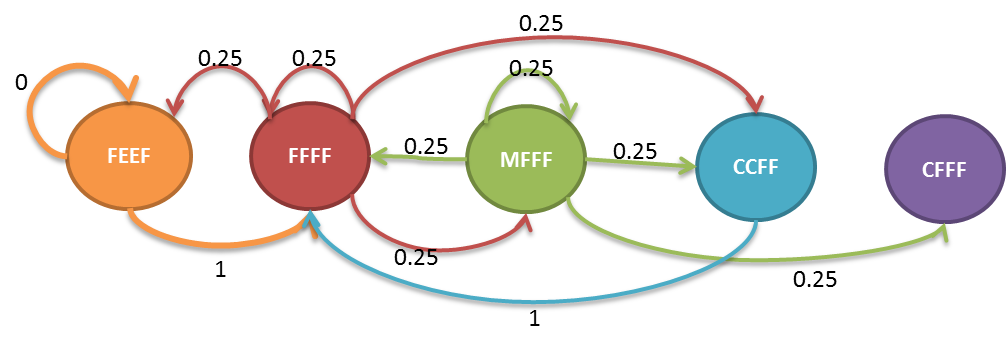
\includegraphics[scale=0.45]{mcc}
  \caption{Simplified transitional matrix}
  \label{fig:transitional-matrix}
\end{figure}


% I am planning whether to add some more stuff about Markov Chain or
% not. Since, well, the OUTLINE of Mrs. Haleimah's thesis is
% unclear. Even if you do not have romance, you should focus on your
% research. I have been a bachelor for a long long time.

\section{Simulation}
\label{sec:simulation}

% This is the simulation part. Never too easy to write a high quality
% paper. But I do not want to say anything BAD about local people.
We carry out the simulation by creating a building model and changing corresponding
parameters with eQuest. The model is a two story office building
with a total floor area of $232m^{2}$. Each floor is divided into four
office zones with a floor area of $40m^{2}$ each. Windows are placed on
the north, east and west walls of the building with overhangs having a
projection factor (overhang depth/window height) of $0.6$. Two doors
are placed on the north and east sides of the building. Windows and
doors are not specified on the south wall to minimize heat gain
through radiation. The window to gross wall area is kept at 29\%. The
cooling system is manually configured to match what is being used
in our institute.


\section{Results}
\label{sec:results}
We adopt two control cases to see their effects on the model. For one
thing, we use a fixed set-point for air conditioning system while
applying a dynamic occupancy schedule generated from MC model. We do
this because the initial building design guide assumes a maximum
occupancy throughout the weekdays, which is far from being trustworthy
according to our observations. For another, we apply the more
authentic schedule alongside with a dynamic set-point that varies
according to the occupancy states. The more populated a zone is, the
lower set-point it will get. Our simulation result is shown in
Figure~\ref{fig:energy-consumption}. The optimum saving is 22.1\% for
month July. 

\begin{figure}[!tb]
  \centering
  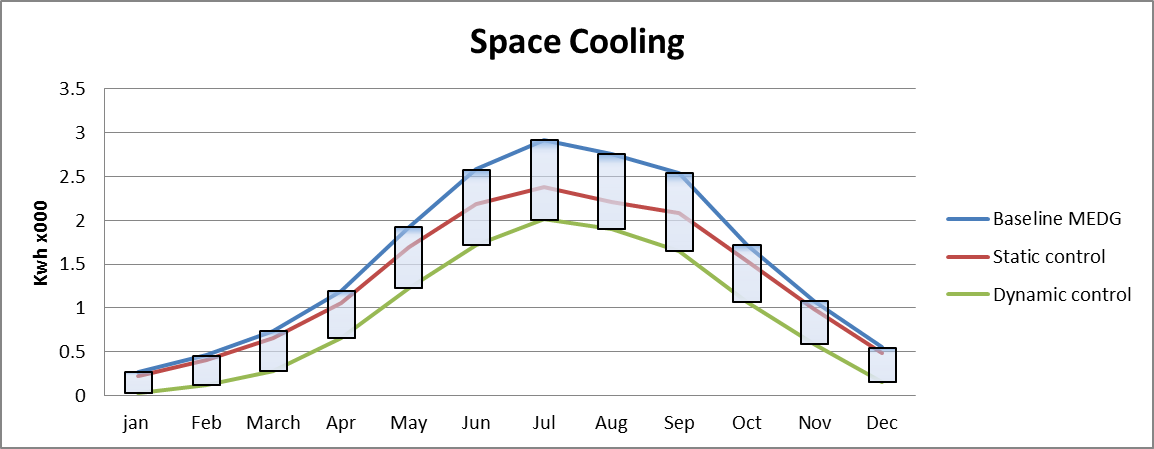
\includegraphics[scale=0.35]{sc}
  \caption{Energy consumption of 3 different control methods}
  \label{fig:energy-consumption}
\end{figure}




% \section{Related Works}
% \label{sec:related-works}


% Comment: I know till now this project sucks. Well, I am not the
% ``main contributor'' and ...



\section{Conclusion and Future Work}
\label{sec:concl-future-work}
We are making those heavily energy-consuming buildings at Masdar
Institute more smart by developing wireless sensor networks to
dynamically control the HVAC system. For now, we have a Kinect-based
mobility tracking system to tell exactly there are how many people in
each zone of an open lab. We build a model using Markov Chain to
predict the likelihood of each zone's next state. And we have
conducted several simulations to see the energy reduction. We plan to
modify our MC model so that it will be more accurate since we have so
many equal probabilities. We will implement the full-scaled experiment
on a field station once everything is settled. 









% \bibliographystyle{plain}
% \bibliography{sigproc}
{\scriptsize
\begin{thebibliography}{1}

\bibitem{ref:Erickson:2010}
Varick~L. Erickson and Alberto~E. Cerpa.
\newblock Occupancy based demand response hvac control strategy.
\newblock In {\em Proceedings of the 2Nd ACM Workshop on Embedded Sensing
  Systems for Energy-Efficiency in Building}, BuildSys '10, pages 7--12, 2010.

\bibitem{ref:Erickson:2009}
Varick~L. Erickson, Yiqing Lin, Ankur Kamthe, et~al.
\newblock Energy efficient building environment control strategies using
  real-time occupancy measurements.
\newblock In {\em Proceedings of the First ACM Workshop on Embedded Sensing
  Systems for Energy-Efficiency in Buildings}, BuildSys '09, pages 19--24,
  2009.

\bibitem{ref:Wang2011}
Chuang Wang, Da~Yan, and Yi~Jiang.
\newblock A novel approach for building occupancy simulation.
\newblock {\em Building Simulation}, 4(2):149--167, 2011.

\end{thebibliography}

}

\balancecolumns

\end{document}


% End of the day
% Successfully ``manage energy'' in buildings. What the heck am I
% reading and writing.
% I have to take part in the next BIG meeting with several
% professors. If possible, I would put forward a plan on HOW TO do
% those smart building buddies.

% Do not rush. Take time and show those reviewers what the heck you
% are doing and to which degree you plan to achieve.